
    \begin{abstract_online}{Temperature Dependent Interaction of Soft Repulsive Wall with the Thermotropic Liquid Crystals }{%
        \underline{J. Kaur}, D. Deb}{%
        }{%
        School of Physics & Materials Science, Thapar Institute of Engineering & Technology, Patiala,Punjab-147004, India}
    Using computer simulations, the effect of soft repulsive wall on a system comprising of thermotropic liquid crystalline material is studied. We place the walls perpendicular to the z-axis at the ends of an anisotropic box with the periodic boundary conditions along x and y axes. Here, the wall interaction strength, temperature and density are the control parameters. We analyzed the effect of temperature on the system confined by the wall at different number densities. Within a limited range of temperatures, we observe that temperature is actually a good control parameter in the system. Moreover, the effect of wall on the system is more pronounced at low number densities. Below are the snapshots of wetting of walls with the bulk liquid crystalline phases at the same denity and at two temperatures with $T=0.8$ (left side) and $T=1.0$ (right side). \begin{center}  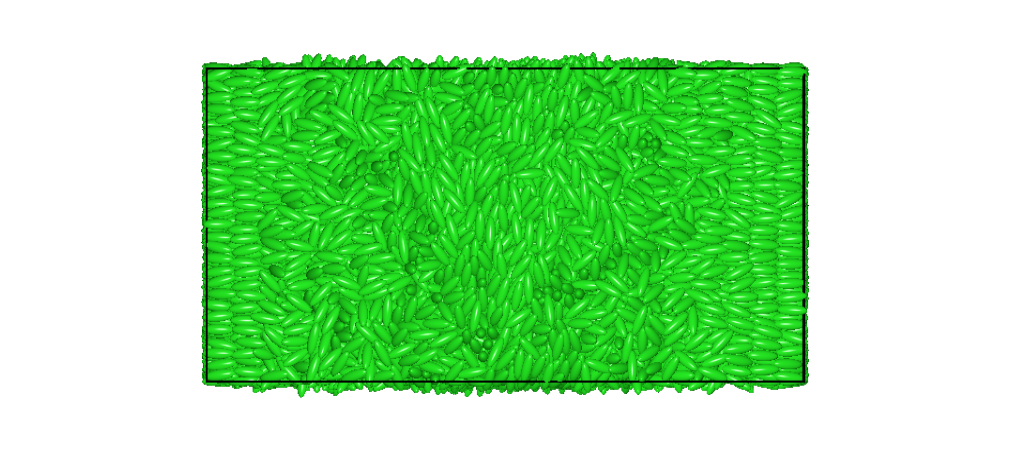
\includegraphics[width=\linewidth]{abstracts/txt/figures/jagroop1.png}  \caption{\textbf{Figure 1:} At $T=0.8$ and $\rho=0.3137$, the bulk (center of the box) phase is the isotropic liquid but the order of the particles away from bulk and close the walls are changed and observed to form layers parallel to the walls.}  \end{center}  \begin{center}  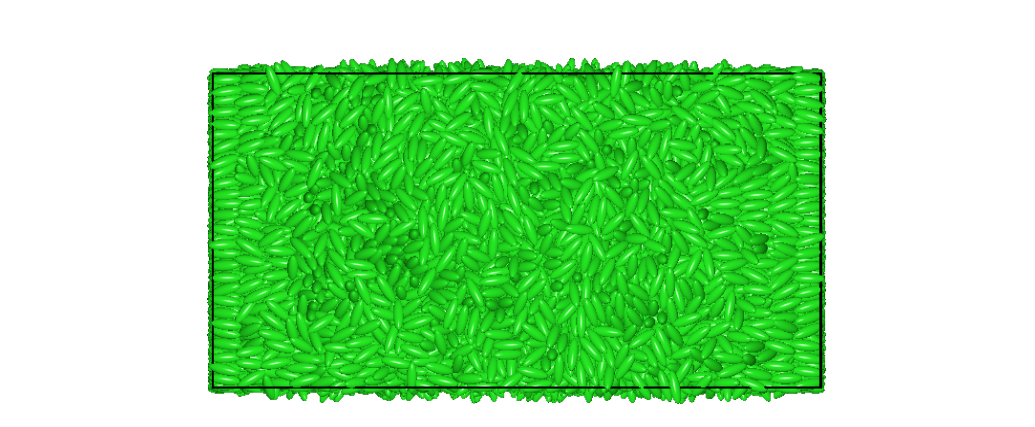
\includegraphics[width=\linewidth]{abstracts/txt/figures/jagroop2.png}  \caption{\textbf{Figure 2:} At $T=1.0$ and $\rho=0.3137$, the bulk (center of the box) phase is the isotropic liquid but the order of the particles away from bulk and close the walls are changed and observed to form layers parallel to the walls. Here the number of layers formed near the wall is less than that of $T=0.8$.}  \end{center}  
    
        \textbf{References} \newline{}[1] K. Binder, et al., J. Stat. Phys., 110 (2003), 1411–1514.\newline{}[2] J. T. Brown, et al., Phys. Rev. E, 57 (1998), 6685-6699 .\newline{}[3] K. Binder, et al., J. Chem. Phys., 145 (2016), 211701.\newline{}[4] E. de Miguel, Mol. Phys., 100 (2002), 2449-2459.
    \end{abstract_online}
    